\documentclass[a4paper,oneside,reqno]{amsart}

\input{../../../../cambridge-macros.tex}

%    Set assignment information here
\newcommand{\authorname}{Feynman Liang}
\newcommand{\coursename}{MLSALT 8: Statistical Machine Translation}
\newcommand{\assignmentname}{Practical 3: Hierarchical Phrase-based Translation
with alternative grammars}

\begin{document}

\title{\coursename\\\assignmentname}

\author{\authorname}
\date{\today}

\maketitle

\section{Preliminary Questions}
\begin{enumerate}[label=\arabic*.]
  \item The language model probability is not included as a feature in the
    rulefile because it is defined for $N$-grams over the target language
    (i.e.\ English). This means that they can only be applied when:
    \begin{enumerate}
      \item A complete sequence of terminals has been derived and no
        non-terminals are remaining
      \item The identity of the previous $N-1$ words is known
    \end{enumerate}
    Rules containing non-terminals or yielding less than $N$ terminal symbols
    do not satisfy these requirements, hence it doesn't make sense to assign
    them a language model score.

    The language model scores could be included if:
    \begin{enumerate}
      \item The language model is a $1$-gram model, in which case the language
        model score of a rule is the joint probability of all the terminals
        derived one step after applying the rule
      \item The degenerate case where the entire sequence of non-terminals is
        derived in a single rule. The score would then be the score of the
        target sentence under the language model.
    \end{enumerate}

  \item % TODO

  \item % TODO
    \begin{lstlisting}[language=bash]
printstrings -n 1000 -u -w --input=output/example/LATS.hyp1/14.fst.gz \
  --print-output-labels 2> /dev/null
    \end{lstlisting}


\end{enumerate}

\section{First part}

\begin{enumerate}[label=\arabic*.]
  \item
    We translate the 30 sentences with grammar A:
    \begin{lstlisting}[language=bash]
hifst $DIR/configs/basic+params.features \
  --textinput=$DIR/input/test30.spa.idx \
  --rulefile=$GRAMA/r.?.gz \
  --lm=$DIR/lm/test30.news-newscomm.eng.4g/G/?.G.gz --lmn=4 \
  --range=1:30 \
  --latoutputfst=output/example/LATS.A/?.fst.gz

printstrings --r=1:30 --input=output/example/LATS.A/?.fst.gz \
  --output=outA --label-map=$SUNMAP
    \end{lstlisting}
    and grammar B:
    \begin{lstlisting}[language=bash]
hifst $DIR/configs/basic+params.features \
  --textinput=$DIR/input/test30.spa.idx \
  --rulefile=$GRAMB/r.?.gz \
  --lm=$DIR/lm/test30.news-newscomm.eng.4g/G/?.G.gz --lmn=4 \
  --range=1:30 \
  --latoutputfst=output/example/LATS.B/?.fst.gz

printstrings --r=1:30 --input=output/example/LATS.B/?.fst.gz \
  --output=outB --label-map=$SUNMAP
    \end{lstlisting}
    During this process, we found that the run with grammar B was significantly slower
    than the run with grammar A.

    Computing BLEU scores:
    \begin{lstlisting}[language=bash]
print "Scoring grammar A:"
ScoreBLEU.sh \
  -t outA \
  -r $DIR/reference/test30.eng
 BLEU score = 0.3515 (0.3515 * 1.0000) for system "1"
 faster

print "Scoring grammar B:"
ScoreBLEU.sh \
  -t outB \
  -r $DIR/reference/test30.eng
    \end{lstlisting}
    We found that Grammar A attains a BLEU score of $0.3515$ while grammar B
    achieves $0.3861$.

    % TODO: post-process the hypotheses?

  \item
    % TODO
    \begin{enumerate}[label=(\alph*)]
      \item
      \item
    \end{enumerate}

  \item
    Some main differences include:
    \begin{enumerate}
      \item A has 104 rules B has 321
      \item A's rules only contain word and phrasal translations; hiero rules
        (i.e.\ productions with both terminals and non-terminals in the yield)
        are absent.  This means that A cannot model arbitrarily long context
        (i.e.\ has as distortion limit) and is equivalent in expressivity to a
        phrase-based SMT system.

        In contrast, B contains hiero rules out of the $X$ non-terminal and
        hence implement hierarchical phrases, which have greater generality
        but also increased computational complexity.
    \end{enumerate}

    These differences can help explain differences in translation. For reference,
    sentence 27:
    \begin{verbatim}
y después llegó la época americana .
    \end{verbatim}
    is translated uder grammar A to:
    \begin{verbatim}
<s> and then came the time american . </s>
    \end{verbatim}
    while under grammar B is translated to:
    \begin{verbatim}
<s> and then came the american era . </s>
    \end{verbatim}

    The grammar A translation appears to translate the sentence word-for-word,
    translationg ``epoca'' literally to time because it failed to account for
    the context. In contrast, grammar B correctly accounts for the context,
    translating ``epoca americana'' to ``american era.''

    The reason why grammar B is able to account for context lies in the presence
    of non-terminals in its yields, ultimately allowing it to achieve
    a significantly higher BLEU score. On the other hand, it also explains
    why translating under grammar B takes more time than grammar A: the presence
    of non-terminals significantly increases the complexity of decoding because
    it leverages the full generality of Hierarchical Phrase Based Translation.

  \item
    \autoref{fig:27-a-tree} and \autoref{fig:27-b-tree} show the derivation
    trees for sentences 27 under rulesets A and B respectively.
    \begin{figure}[h!]
      \begin{center}
        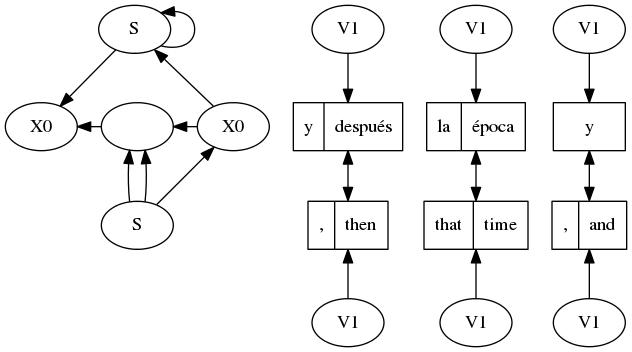
\includegraphics[scale=0.5]{../output/tree27Advn1.jpg}
      \end{center}
      \caption{Sentence 27 derivation tree under ruleset A}
      \label{fig:27-a-tree}
    \end{figure}
    \begin{figure}[h!]
      \begin{center}
        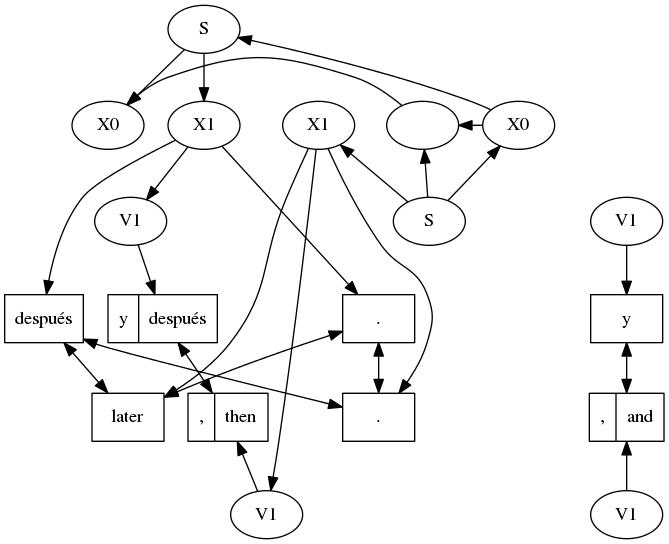
\includegraphics[scale=0.5]{../output/tree27Bdvn1.jpg}
      \end{center}
      \caption{Sentence 27 derivation tree under ruleset B}
      \label{fig:27-b-tree}
    \end{figure}
    % TODO: relate to previous questions

  \item Aligning the 30 sentences towards respective English references:
    \begin{lstlisting}[language=bash]
hifst $DIR/configs/basic+params.features \
  --textinput=$DIR/input/test30.spa.idx \
  --rulefile=$GRAMA/r.?.gz \
  --lm=$DIR/lm/test30.news-newscomm.eng.4g/G/?.G.gz --lmn=4 \
  --range=1:30 \
  --latoutputfst=output/example/LATS.A.towards_ref/?.fst.gz \
  --towardsreference=$DIR/reference/test30/r.?.eng.idx
hifst $DIR/configs/basic+params.features \
  --textinput=$DIR/input/test30.spa.idx \
  --rulefile=$GRAMB/r.?.gz \
  --lm=$DIR/lm/test30.news-newscomm.eng.4g/G/?.G.gz --lmn=4 \
  --range=1:30 \
  --latoutputfst=output/example/LATS.B.towards_ref/?.fst.gz \
  --towardsreference=$DIR/reference/test30/r.?.eng.idx
    \end{lstlisting}
    Comparing the number of input sentences generating the reference for each
    grammar:

    % TODO: by examining the resulting output transducers!
    \begin{lstlisting}
integer Acnt=0
integer Bcnt=0
for i in {1..30}; do
  integer newA=$(printstrings -n 500000 -u -w --input=output/example/LATS.A.towards_ref/$i.fst.gz \
    2>/dev/null \
    | wc -l)
  integer newB=$(printstrings -n 500000 -u -w --input=output/example/LATS.B.towards_ref/$i.fst.gz \
    2>/dev/null \
    | wc -l)
  print "$i, $newA, $newB"
  Acnt+=newA
  Bcnt+=newB
done
print "Acnt: $Acnt, Bcnt: $Bcnt"
    \end{lstlisting}

    We obtain the results shown in \autoref{tab:inputs-per-ref}.
    \begin{table}[h]
      \begin{tabular}{ccc}
        \toprule
        Sentence \# & \multicolumn{2}{c}{Number inputs generating reference}\\
        & Grammar A & Grammar B \\
        \midrule
        1 & 4     & 8       \\
        2 & 1     & 1       \\
        3 & 1     & 1       \\
        4 & 1     & 1       \\
        5 & 1     & 165     \\
        6 & 1     & 1       \\
        7 & 1     & 8586    \\
        8 & 1     & 1       \\
        9 & 1     & 1       \\
        10& 48    & 122     \\
        11& 1     & 1       \\
        12& 1     & 84      \\
        13& 11070 & 51692   \\
        14& 47    & 83      \\
        15& 1     & 1       \\
        16& 1     & 1       \\
        17& 1     & 1       \\
        18& 1     & 1       \\
        19& 1     & 1       \\
        20& 52    & 166     \\
        21& 1     & 1       \\
        22& 500000& 500000  \\
        23& 2586  & 14030   \\
        24& 1     & 1       \\
        25& 1     & 282     \\
        26& 270   & 658     \\
        27& 1     & 1       \\
        28& 1     & 1       \\
        29& 1     & 1       \\
        30& 1     & 1       \\
        \hline
        Total & 514099 & 575894\\
        \bottomrule
      \end{tabular}
      \caption{Sentences aligned towards their references}
    \end{table}

  \item

  \item

\end{enumerate}

\section{Second part}

\begin{enumerate}[label=\arabic*.]
  \item

  \item
    Aligning the sentences with their English refrence with grammar C:

    \begin{lstlisting}[language=bash]
hifst $DIR/configs/basic+params.features \
  --textinput=$DIR/input/test30.spa.idx \
  --rulefile=$GRAMC/r.?.gz \
  --lm=$DIR/lm/test30.news-newscomm.eng.4g/G/?.G.gz --lmn=4 \
  --range=1:30 \
  --latoutputfst=output/example/LATS.C.towards_ref/?.fst.gz \
  --towardsreference=$DIR/reference/test30/r.?.eng.idx
    \end{lstlisting}

    Comparing the number of input sentences generating the reference
    for grammars B and C:

    \begin{lstlisting}[language=bash]
integer Bcnt=0
integer Ccnt=0
for i in {1..30}; do
  integer newB=$(printstrings -n 500000 -u -w --input=output/example/LATS.B.towards_ref/$i.fst.gz \
    2>/dev/null \
    | wc -l)
  integer newC=$(printstrings -n 500000 -u -w --input=output/example/LATS.C.towards_ref/$i.fst.gz \
    2>/dev/null \
    | wc -l)
  print "$i, $newB, $newC"
  Bcnt+=newB
  Ccnt+=newC
done
print "Bcnt: $Bcnt, Ccnt: $Ccnt"
    \end{lstlisting}

    We obtain the results % TODO
    \begin{verbatim}
    \end{verbatim}

  \item
\end{enumerate}

%\bibliographystyle{alpha}
%\nocite{*}
%\bibliography{refs}

%\appendix

%\section{Code Listings}

\end{document}
